\chapter{البرمجة المجزّأة (\textenglish{Modular Programming})}

في هذه المرحلة الثانية، سنكتشف مبادئ متقدّمة في لغة الـ\textenglish{C}
 لن أخفي عليك، هذه المرحلة صعبة الفهم و تحتاج منك التركيز. في نهاية المرحلة، ستكون قادراً على تدبّر أمرك في معظم البرامج المكتوبة بلغة الـ\textenglish{C}. 
في المرحلة التي تليها نتعلّم كيف نفتح نافذة، كيف ننشئ لعبة ثنائية الأبعاد\dots إلخ.

لحدّ الآن عملنا في ملف واحد سمّيناه
\InlineCode{main.c}.
كان أمراً مقبولاً لحدّ الآن لأن برامجنا كانت صغيرة، لكنها ستصبح في القريب العاجل مركّبة من عشرات، لن أقول من مئات الدوال، و إن كنت تريد وضعها كلّها في نفس الملف، فإن هذا الأخير سيصبح ضخماً جداً. لهذا السبب تم اختراع ما نسمّيه بالبرمجة المجزّأة. المبدأ سهل : بدل أن نضع كل الشفرة المصدرية في ملف واحد
\InlineCode{main.c}
، سنقوم بتفريقها إلى عدة ملفات.

\section{النماذج (\textenglish{Prototypes})}

لحدّ الآن، كنت عندما تنشئ دالة، أطلب منك وضعها قبل الدالة الرئيسية
\InlineCode{main}
. لماذا ؟

لأن للترتيب أهمية حقيقية هنا : فإن قمت بوضع الدالة قبل الـ\InlineCode{main}
في الشفرة المصدرية، سيقرؤها الجهاز و يتعرف عليها. حينما تقوم باستدعاء الدالة داخل الـ\InlineCode{main}
، سيعرفها الجهاز و يعرف أيضاً أين يبحث عليها.\\
بالعكس، لو تضع الدالة بعد الـ\InlineCode{main}
، لن يعمل البرنامج لأن الجهاز لم يتعرّف بعد على الدالة. جرّب ذلك و سترى.

\begin{question}
  لكنه تصميم سيّء نوعاً ما، أليس كذلك ؟
\end{question}

أنا متفق معك ! لكن انتبه المبرمجون لهذه النقطة قبلك و عملوا على حلّ المشكل.

بفضل ما سأعلمك إياه الآن، ستتمكن من الدوال في أي ترتيب كان في الشفرة المصدرية، هكذا لن تقلق من هذه الناحية.

\subsection{استعمال النموذج للتصريح عن دالة}

سنقوم بتصريح دوالنا للحاسوب، و هذا بكتابة ما نسميه بـ\textbf{النماذج}
.لا تنبهر بهذا الاسم، إنه يخبّئ معلومة بسيطة جداً.

تأمل في السطر الأول من دالتنا
\InlineCode{rectangleSurface}

\begin{Csource}
double rectangleSurface(double width, double height)
{
	return width * height;
}
\end{Csource}

قم بنسخ السطر الأول
(\InlineCode{double rectangleSurface...})
المتواجد أعلى الشفرة المصدرية (مباشرة بعد تعليمات التضمين
\InlineCode{\#include}
). أضف
\textbf{فاصلة منقوطة}
في نهاية هذا السطر.\\
و هكذا يمكنك أن تضع الدالة الخاصة بك
\InlineCode{rectangleSurface}
بعد الدالة
\InlineCode{main}
ان أردت !

هذا ما يجب أن تكون عليه الشفرة المصدرية :

\begin{Csource}
#include <stdio.h>
#include <stdlib.h>
// The next line represents the prototype of the function rectangleSurface :
double rectangleSurface(double width, double height);
int main(int argc, char *argv[])
{
	printf("width = 5 and height = 10. Surface = %f\n", rectangleSurface(5, 10));
	printf("width = 2.5 and height = 3.5. Surface = %f\n", rectangleSurface(2.5, 3.5));
	printf("width = 4.2 and height = 9.7. Surface = %f\n", rectangleSurface(4.2, 9.7));

	return 0;
}
// Now, we can put our function wherever we want in the source code :
double rectangleSurface(double width , double height )
{
	return width * height ;
}
\end{Csource}

الشيء الذي تغيّر هنا هو إضافة النموذج أعلى الشفرة المصدرية.\\
النموذج هو عبارة عن إشارة للجهاز، يوحي إليه بوجود دالة تسمى
\InlineCode{rectangleSurface}
و التي تأخذ معاملات إدخال معينة و تُرجِع مخرجا من نوع أنت من تحدده.  هذا يساعد الجهاز على تنظيم نفسه.

بفضل ذلك السطر، يمكنك الآن وضع دوالك في أي ترتيب كان دون أي تفكير زائد.

أكتب دائما النموذج الخاص بدوالك. البرامج التي ستكتبها من الآن و صاعداً ستصبح أكثر تعقيداً و تستعمل الكثير من الدوال : من الأحسن أن تتعلّم منذ الآن العادة الجيدة  بوضع نموذج لكل دالة في الشفرة المصدرية.

كما ترى، الدالة
\InlineCode{main}
لا تملك أي نموذج، و كمعلومة فهي الوحيدة التي لا تملك نموذجاً ! لأن الجهاز يعرفها (فهي نفسها مكررة في جميع البرامج).

عليك أن تعرف أنه في سطر النموذج، لست مضطراً إلى تحديد المعاملات التي تتلقاها الدالة كمدخل. الجهاز يحتاج أن يتعرّف إلى نوع المداخل فقط.

يمكننا أن نكتب ببساطة :

\begin{Csource}
double rectangleSurface (double, double);
\end{Csource}

و مع ذلك، فالطريقة التي أريتك إياها أعلاه تعمل أيضاً. الشيء الجيد فيها هو أن كلّ ما عليك فعله هو نسخ و لصق السطر الأول الخاص بالدالة مع إضافة فاصلة منقوطة (طريقة سهلة و سريعة).

\begin{critical}
  لا تنس
\underline{أبدا}
وضع فاصلة منقوطة بعد النموذج، هذا يمكّن الحاسوب من التفريق بين النموذج و بداية الدالة.\\
إن لم تفعل، ستعترضك أخطاء غير مفهومة أثناء عملية الترجمة.
\end{critical}

\section{الملفات الرأسية (\textenglish{Headers})}

لحدّ الآن لا نملك غير ملفٍ مصدريٍ واحد في مشروعنا و هو الذي كنّا نسمّيه
\InlineCode{main.c}.

\subsection{عدة ملفات في مشروع واحد}

تطبيقياً، برامجك لن تكون مكتوبة في ملف واحد
\InlineCode{main.c}.
بالطبع يمكن فعل ذلك، لكن لن يكون من الممتع أن تتجوّل في ملف به 10000 سطر (شخصياً أعتقد هذا). و لهذا فإنه في العادة ننشئ العديد من الملفات في المشروع الواحد.
\begin{question}
  عفوا ... ماهو المشروع ؟
\end{question}
لا ! هل نسيت بسرعة ؟ سأعيد الشرح لأنه من اللازم أن نتّفق على هذا المصطلح.

المشروع هو مجموع الملفات المصدرية الخاصة ببرنامجك. لحد الآن برنامجنا لم تتكون إلا من ملف واحد. و يمكنك التحقق من هذا بالنظر في البيئة التطويرية الخاصة بك، غالبا ما يظهر المشروع في القائمة على اليسار (الصورة الموالية) :

\begin{figure}[H]
	\centering
	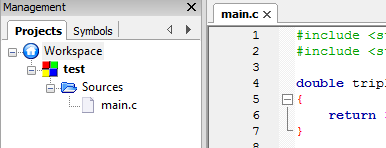
\includegraphics[width=0.4\textwidth]{Chapter_II-1_Project}
\end{figure}

كما يمكنك رؤيته في يسار الصورة، هذا المشروع ليس مكوّنا إلا من الملف
\InlineCode{main.c}.

اسمح لي الآن أن أُرِيَكَ صورة لمشروع حقيقي ستقوم به في وقت لاحق من الكتاب : لعبة 
\textenglish{Sokoban} :

\begin{figure}[H]
	\centering
	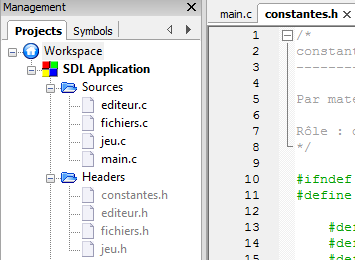
\includegraphics[width=0.4\textwidth]{Chapter_II-1_Project-Sokoban}
\end{figure}

كما ترى، هناك ملفات عديدة. هذا ما يكون عليه المشروع الحقيقي، أي تتواجد به ملفات عديدة في القائمة اليسارية  يمكن التعرّف على الملف
\InlineCode{main.c}
من بين القائمة و الذي يحتوي الدالة
\InlineCode{main}.
بصورة عامة في برامجي، لا أضع إلّا الدالة
\InlineCode{main}
في الـملف
\InlineCode{main.c}.
لمعلوماتك، هذا ليس أمراً إجبارياً، كل واحد ينظّم ملفاته بالشكل الذي يريد. لكن لكي تتبعني جيّداً أنصحك بفعل ذلك.

\begin{question}
  لكن لم يجب عليّ إنشاء ملفات عديدة ؟ و كم من ملف يجب علىّ أن أنشئ في مشروعي ؟
\end{question}

هذا يبقى اختيارك أنت، في الغالب نجمع في نفس الملف المصدري الدوال التي تشترك في الموضوع الذي تعالجه. و هكذا ففي الملف
\InlineCode{editeur.c}
جمعت كلّ الدوال الخاصة ببناء المستوى، و في الملف
\InlineCode{jeu.c}
قمت بتجميع الدوال الخاصة باللعبة نفسها و هكذا ...

\subsection{الملفات \texttt{.c} و \texttt{.h}}

كما يمكنك أن تلاحظ، يوجد نوعان مختلفان من الملفات في الصورة السابقة.

\begin{itemize}
  \item \textbf{ملفات ذات الإمتداد
\InlineCode{.c}}
: الملفات المصدرية، تحتوي الدوال نفسها.
  \item \textbf{ملفات ذات الإمتداد
\InlineCode{.h}}
: تسمى الملفات الرأسية و هي تحتوي النماذج الخاصة بالدوال.
\end{itemize}

عموما، إنه لمن النادر وضع نماذج في الملفات من صيغة
\InlineCode{.c}
مثلما فعلنا للتوّ في الـملف
\InlineCode{main.c}
(إلا إذا كان برنامجك صغيرا).

من أجل كل ملف
\InlineCode{.c}
هناك ملف مكافئ له، و الذي يحتوي نماذجا للدوال الموجودة في الملف
\InlineCode{.c}،
تمعّن في الصورة السابقة.

\begin{itemize}
  \item هناك
\InlineCode{editeur.c}
(الشفرة الخاصة بالدوال) و
\InlineCode{editeur.h}
(ملف النماذج الخاصة بالدوال).
  \item هناك
\InlineCode{jeu.c}
و
\InlineCode{jeu.h}.
  \item إلخ.
\end{itemize}

\begin{question}
  لكن كيف يعرف الحاسوب بأن نماذج الدوال موجودة في ملف آخر خارج الملف
\InlineCode{.c}
؟
\end{question}

يجب عليك تضمين الملف الرأسي
\InlineCode{.h}.
مستعيناً بتوجهات المعالج القبلي.\\
كن مستعداً لأنّي سأعطيك الكثير من المعلومات في وقت قصير.

كيف نقوم بتضمين ملف رأسي ؟ أنت تجيد فعل ذلك لأنك قمت بذلك من قبل.

أنظر مثالاً من بداية الملف
\InlineCode{jeu.c} :

\begin{Csource}
#include <stdlib.h>
#include <stdio.h>
#include "jeu.h"
void play(SDL_Surface* screen)
{
// ...
\end{Csource}

التضمين يتم عن طريق توجيهات المعالج القبلي
\InlineCode{\#include}
التي يجدر بك أن تكون قد تعلّمتها من قبل.\\
تمعن في التالي :

\begin{Csource}
#include <stdlib.h>
#include <stdio.h>
#include "jeu.h" // We include jeu.h
\end{Csource}

قمنا بتضمين ثلاثة ملفات من صيغة
\InlineCode{.h}
و هي :
\InlineCode{stdio}، \InlineCode{stdlib} و \InlineCode{jeu}.\\
لاحظ الفرق : الملفات التي قمت بإنشائها ووضعها في الـمجلّد الخاص بمشروعك يجب أن تكون مضمّنة بإشارات الاقتباس
(\InlineCode{"jeu.h"})
بينما ملفات المكتبات (التي توجد عادة في البيئة التطويرية الخاصة بك) تكون مضمّنة بعلامات الترتيب
(\InlineCode{<stdio.h>}).

تستعمل إذا :

\begin{itemize}
  \item علامتي الترتيب
\InlineCode{< >}
: لتضمين الملفات المتواجدة في المجلّد
\InlineCode{include}
الخاص بالبيئة التطويرية.
  \item علامتي الاقتباس
\InlineCode{" "}
 : لتضمين  الملفات المتواجدة في مجلّد المشروع (و غالبا بجانب الملفات
\InlineCode{.c}).
\end{itemize}

الأمر
\InlineCode{\#include}
يطلب إدخال محتوى ملف معيّن في الملف
\InlineCode{.c}
فهي تعليمة تقول :"أدخل الملف
\InlineCode{jeu.h}
هنا" مثلا .

\begin{question}
  و في الملف
\InlineCode{jeu.h}
ماذا نجد ؟
\end{question}

لا نجد إلا نماذج خاصة بدوال الملف
\InlineCode{jeu.c} !

\begin{Csource}
void play(SDL_Surface* screen);
void movePlayer(int map[][NB_BLOCS_HEIGHT], SDL_Rect *pos, int direction);
void moveBox(int *firstBox, int *secondeBox);
\end{Csource}

هكذا يعمل المشروع الحقيقي !

\begin{question}
  ما الهدف من وضع نماذج في ملفات من نوع
  \InlineCode{.h}
  ؟
\end{question}

السبب بسيط للغاية، عندما تستدعي دالة في الشفرة المصدرية الخاصة بك، ينبغى لجهازك أن يكون متعرفا عليها من قبل، و يعرف كم من المعاملات تستعمل...إلخ. إن هذا هو الهدف وراء وجود النماذج، إنه دليل الاستخدام الخاص بالدالة بالنسبة للجهاز.

كلّ هذا هو مسألة تنظيم، عندما تضع نماذجك في ملفات
\InlineCode{.h}
(ملفات رأسية) مضمّنة في أعلى الملفات
\InlineCode{.c}،
سيعرف جهازك طريقة استخدام الدوال الموجودة في الملف ما إن يبدأ في قراءته.

عند القيام بهذا، لن يكون عليك القلق حيال الترتيب الذي ستكون عليه دوالك في الملفات
\InlineCode{.c}.
إذا كنت قمت الآن بإنشاء برنامج صغير يحتوي على دالتين أو ثلاث يمكنك أن تفكّر أنه من الممكن للبرنامج أن يتشغل دون وجود النماذج، لكن هذا لن يستمر طويلا ! فما إن يكبر البرنامج و إن لم تنظّم النماذج في ملفات رأسيّة فستفشل الترجمة دون أدنى شك.

\begin{information}
  عندما تستدعي دالة متواجدة في الملف
  \InlineCode{functions.c}
  إنطلاقا من الملف
  \InlineCode{main.c}
  سيكون عليك تضمين النماذج الخاصة بالملف
  \InlineCode{functions.c}
  في الملف
  \InlineCode{main.c}
  يجب إذن وضع
  \InlineCode{\#include "functions.h"}
  في أعلى الـملف
  \InlineCode{main.c}.\\
  تذكر هذه القاعدة : "في كلّ مرة تستدعي الدالة
  \textenglish{X}
  في ملف، يجب عليك إدراج نموذج هذه الدالة في ملفك" هذا ما يسمح للـمترجم بمعرفة ما إن كنت قد استدعيتها بشكل صحيح.
\end{information}

\begin{question}
  كيف أقوم بإضافة ملفات
\InlineCode{.c}
 و
\InlineCode{.h}
 إلى مشروعي ؟
\end{question}

هذا راجع للـبيئة التطويرية التي تستخدمها. لكن المبدأ هو نفسه في جميع البرامج :
\InlineCode{File} / \InlineCode{New} / \InlineCode{Source File}\\
هذا يسمح بإنشاء ملف جديد فارغ. هذا الملف ليس حاليا من النوع
\InlineCode{.c}
ولا
\InlineCode{.h}
أنت من يحدد ذلك أثناء عملية حفظ الملف. قم إذن بحفظه (حتّى و إن كان لا يزال فارغا !) و هنا يطلب منكم إدخال اسم للملف، يمكنك هنا اختيار صيغة الملف :

\begin{itemize}
  \item إذا سميته
\InlineCode{file.c}
فسيكون بامتداد
\InlineCode{.c}.
  \item إذا سميته
\InlineCode{file.h}
فسيكون بامتداد
\InlineCode{.h}.
\end{itemize}

هذا سهل. قم بحفظ الملف في المجلّد أين تتواجد باقي الملفات الخاصة بمشروعك (نفس المجلّد أين يتواجد الملف
\InlineCode{main.c}). عموما كل ملفات المشروع تقوم بحفظها في نفس المجلّد سواء كانت ذات صيغة
\InlineCode{.c}
أو
\InlineCode{.h}.

مجلّد المشروع في النهاية سيكون مثل هذا :

\begin{figure}[H]
	\centering
	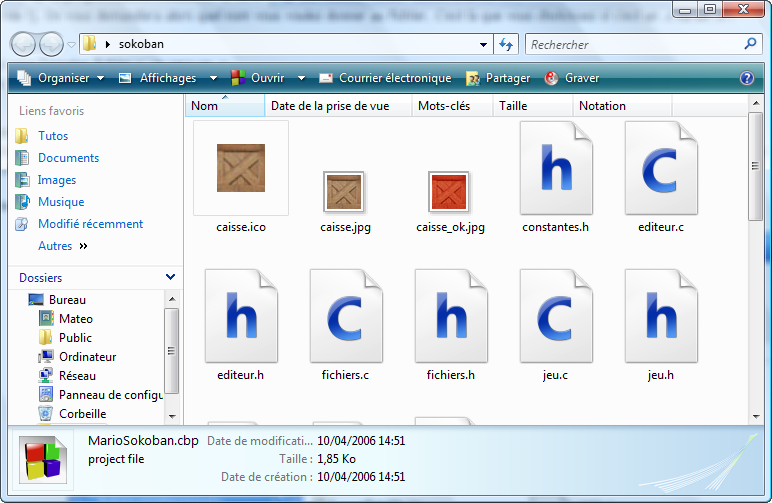
\includegraphics[width=0.8\textwidth]{Chapter_II-1_Project-Sokoban-Folder}
\end{figure}

الملف الذي أنشأته محفوظ لكن لم تتم إضافته إلى مشروعك بعد !\\
لإضافته قم بالنقر يمينا على القائمة أيسر الشاشة (الخاصة بملفات المشروع) و اختر
\InlineCode{Add files}
كالتالي :

\begin{figure}[H]
	\centering
	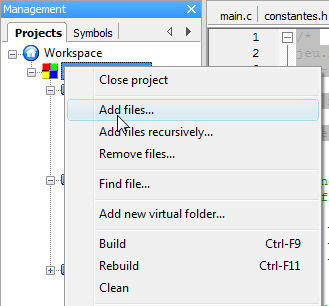
\includegraphics[width=0.4\textwidth]{Chapter_II-1_Project-Add-File}
\end{figure}

ستظهر لك نافذة تطلب منك اختيار الملفات التي تريد أن تدخلها للمشروع، اختر الملف الذي قمت بإنشاءه، للتو، و سيتم إدخاله أخيرا في المشروع.  ستجده حاضراً في القائمة اليسارية !

\subsection{الـ\texttt{include} الخاصّة بالمكتبات النموذجية}

يفترض أنّ لديك سؤالا يدور في رأسك الآن\dots\\
إذا ضمّنا الملفات
\InlineCode{stdio.h}
و
\InlineCode{stdlib.h}
فهذا يعني أنهما موجودان في مكان ما و يمكننا البحث عنهما، أليس كذلك~؟

نعم بالطبع !\\
يفترض أنهما مسطبان في المكان الذي تتواجد به البيئة التطويرية الخاصة بك، بالنسبة للبيئة
\textenglish{Code::Blocks}
أجدهم هنا :

\InlineCode{C:\textbackslash Program Files\textbackslash CodeBlocks\textbackslash MinGW\textbackslash include}

على العموم يجب البحث عن مجلد يحمل اسم
\InlineCode{include}.\\
بداخله تجد كمّا هائلا من الملفات، و هي ملفات رأسية
(\InlineCode{.h})
خاصة بمكتبات نموذجية أي مكتبات متوفرة في كل مكان (سواء في 
\textenglish{Windows}
أو
\textenglish{\mbox{Mac OS X}}
أو 
\textenglish{\mbox{GNU/Linux}}\dots)،
و ستجد داخلها الملفات
\InlineCode{stdio.h}
و
\InlineCode{stdlib.h}
مع ملفّات أخرى.

يمكنك فتحها إذا أردت، لكن ستتفاجئ بالعديد من الأشياء التي لم أدرّسها لك من قبل خاصة بما يتعلق ببعض توجيهات المعالج القبلي. يمكنك أن تلاحظ بأن الملف مليء بنماذج لدوال نموذجية مثل
\InlineCode{printf}.

\begin{question}
  حسناً، الآن عرفت أين أجد نماذج الدوال النموذجية لكن ألا يمكنني رؤية الشفرة المصدرية الخاصة بالدوال ؟ أين هي الملفات
\InlineCode{.c}
؟
\end{question}

إنها غير موجودة أساسا ، لأنها مترجمة (إلى ملفات ثنائية
(\textenglish{binary files})،
يعني إلى لغة الحاسوب). و لهذا فإنه من المستحيل أن تقرأها.

يمكنك إيجاد الملفات المترجمة في المجلّد المسمى
\InlineCode{lib}
(و الذي هو اختصار لكلمة
\InlineCode{library}
أي مكتبة)، بالنسبة لي هي موجودة في المسار :

\InlineCode{C:\textbackslash Program Files\textbackslash CodeBlocks\textbackslash MinGW\textbackslash lib}

ملفات المكتبات المترجمة لها الصيغة
\InlineCode{.a}
في البيئة
\textenglish{Code::Blocks}
و التي تستخدم
\InlineCode{mingw}
كمترجم. و لها صيغة
\InlineCode{.lib}.
في برنامج
\textenglish{Visual C++}
الذي يستخدم المترجم
\InlineCode{Visual}.
لا تحاولوا قراءتها لأنها غير قابلة للقراءة من طرف إنسان عادي.

باختصار، يجب عليك أن تضمّن الملفات الرأسية
\InlineCode{.h}
في الملفات
\InlineCode{.c}
تتمكن من استخدام الدوال النموذجية مثل
\InlineCode{printf}
و كما تعرف فالجهاز على اطلاع على النماذج فهو يعرف ما إن كنت قد طلبت الدوال بشكل صحيح (إن لم تنس أحد المعاملات مثلا).

\section{الـترجمة المنفصلة}

الآن و بعدما عرفت أن المشروع مبنى على أساس ملفات مصدرية عديدة، يمكننا الدخول الآن في تفاصيل عملية الترجمة فلحد الآن لم نر سوى مخطط مبسط عنها.

سأعطيك الآن مخططا مفصلا عنها و من المستحسن أن تحفظه عن ظهر قلب :

\begin{figure}[H]
	\centering
	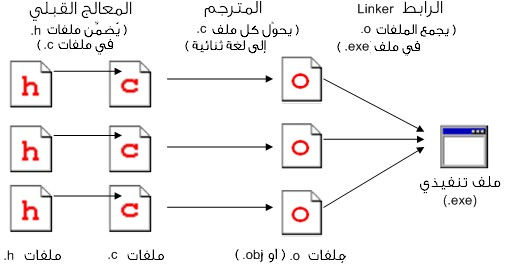
\includegraphics[width=0.7\textwidth]{Chapter_II-1_Compilation-Schema}
\end{figure}

هذا مخطط حقيقي عمّا يجري بالضبط أثناء التجميع و سأشرحه لك :

\begin{enumerate}
  \item \textbf{المعالج القبلي} :
المعالج القبلي هو برنامج ينطلق قبل عملية الترجمة و هو مخصص للقيام بتشغيل تعليمات نطلبها منه عن طريق ما سميناه بتوجيهات المعالج القبلي، و هي الأسطر الشهيرة التي تبدأ يإشارة
\InlineCode{\#}.

لحد الآن توجيهة المعالج القبلي الوحيدة الّتي نعرفها هي
\InlineCode{\#include}
و الّتي تسمح بإدراج ملف في ملف آخر. طبعا للمعالج القبلي مهام أخرى سنتعرف إليها لاحقا لكن ما يهمنا الآن هو ما أعطيتك إياه.
المعالج القبلي يقوم إذن بـ"استبدال" أسطر
\InlineCode{\#include}
بملفات أخرى نحددها، فهو يضمّن داخل كل الملفات
\InlineCode{.c}
الملفات
\InlineCode{.h}
التي نعينها و نطلب منه تضمينها في السابقة.
  \item \textbf{الترجمة} : هذه الخطوة المهمة التي تسمح بتحويل ملفاتك إلى شفرات ثنائية مفهومة للحاسوب. فالمترجم ييقوم بتجميع الملفات
\InlineCode{.c}
واحدا بواحدا حتى ينهيها جميعها، و لضمان ذلك يجب أن تكون كل الملفات موجودة في المشروع (بحيث تظهر في القائمة اليسارية).

سيقوم المترجم بتوليد ملف
\InlineCode{.o}
أو
\InlineCode{.obj}
و هذا راجع لنوع المترجم و هي ملفات ثنائية مؤقتة، و على أي حال تحذف هذه الملفات في نهاية الـترجمة و لكن بتعديل الخيارات يمكنك الإبقاء عليها لكن لكن يكون هناك من داع.
  \item \textbf{إنشاء الروابط} :
محرر الروابط
(\textenglish{Linker})
هو برنامج يعمل على جمع الملفات الثنائية من نوع
\InlineCode{.o}
في ملف واحد كبير : الملف التنفيذي النهائي ! هذا الملف يحمل الصيغة
\InlineCode{.exe}
في الويندوز. إن كنت تملك نظام تشغيل آخر فسيأخذ الصيغة المناسبة له.
\end{enumerate}

و هكذا تكون قد تعرفت على الطريقة الحقيقية لعمل الترجمة. كما قلتها و أكررها المخطط أعلاه مهم للغاية، فهو يفرق بين مبرمج يقوم بجمع و نسخ الشفرة المصدرية دون فهم و بين مبرمج يعرف تماما ما عليه فعله !

معظم الأخطاء تحدث في الـترجمة و قد تأتي من محرر الروابط و هذا يعني أنه لم يتمكن من تجميع كل الملفات
\InlineCode{.o}
بطريقة صحيحة (ربمّا لفقدان إحداها).

لا يزال المخطط أعلاه غير كامل، إذ أن المكتبات لم تظهر فيه ! إذن كيف تحدث العملية عندما نستخدم مكتبات برمجية ؟

تبقى بداية المخطط هي نفسها، لكن يقوم محرر الروابط بأعمال أخرى، سيقوم بتجميع ملفاتك
\InlineCode{.o}
(المؤقتة) مع مكتبات جاهزة تحتاجها 
(\InlineCode{.a}
أو
\InlineCode{.lib}
وفقا للمترجم) :

\begin{figure}[H]
	\centering
	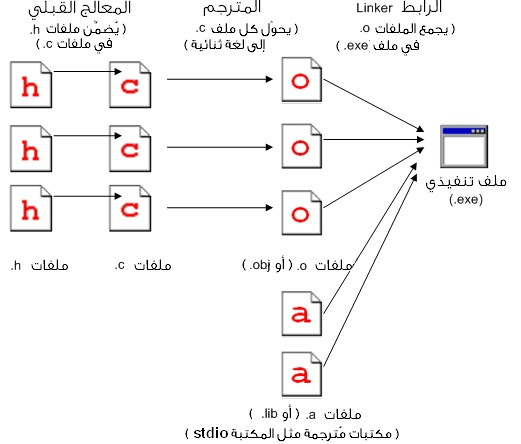
\includegraphics[width=0.7\textwidth]{Chapter_II-1_Compilation-Schema-Libraries}
\end{figure}

هكذا ننتهي و يكون مخططنا هذه المرة كاملا، ملفاتك من المكتبات
\InlineCode{.a}
(أو
\InlineCode{.lib})
يتم تجميعها في الملف التنفيذي مع الملفات
\InlineCode{.o}.

فبهذه الطريقة نتحصل في النهاية على برنامج كامل
100\%
و الذي يحتوي كل التعليمات اللازمة للجهاز لتشرح له كيف يعرض نصّا !\\
كمثال، الدالة
\InlineCode{printf}
توجد في ملف
\InlineCode{.a}
و طبعا سيتم تجميعها مع الشفرة المصدرية الخاصّة بنا في الملف التنفيذي.

لاحقا سنتعلم كيف نستخدم المكتبات الرسومية التي نجدها أيضا في ملفات
\InlineCode{.a}
و تعطي للجهاز تعليمات خاصة بكيفية إظهار نافذة على الشاشة كمثال. لكن طبعا، لن ندرسها الآن ، كلّ شيء في وقته.

\section{نطاق الدوال و المتغيرات}

لننهي هذا الفصل، يجب أن أطلعكم عما يسمى بـ\textbf{نطاق}
المتغيرات و الدوال، سنعرف إمكانية الوصول للدوال و المتغيرات، يعني متى يمكننا استدعاؤها.

\subsection{المتغيرات الخاصة بدالة}

عندما تصرّح عن متغير في داخل دالة يتم حذف هذا المتغير من الذاكرة مع نهاية الدالة.

\begin{Csource}
int triple(int number)
{
	int result = 0; // The variable result is created in the memory
	result = 3 * number;
	return result;
} // The function finished, the variable result is destroyed
\end{Csource}

كلّ متغير تم التصريح عنه في دالة، لا يكون موجودا سوى حينما تكون الدالة في طور الإشتغال.\\
لكن ماذا يعني هذا تحديدا ؟ أنه لا يمكن الوصول إليه من خلال  دالة اخرى !

\begin{Csource}
int triple(int number);
int main(int argc, char *argv[])
{
	printf("The triple of 15 = %d\n", triple(15));
	printf("The triple of 15 = %d",  result); // Error
	return 0;
}

int triple(int number)
{
	int result = 0;
	result = 3 * number;
	return result;
}
\end{Csource}

في الدالة الرئيسية أحاول الوصول إلى المتغير
\InlineCode{result}
و بما أن هذا المتغير تم التصريح عنه داخل الدالة
\InlineCode{triple}
فطبعا لا يمكنني الوصول إليه من خلال الدالة
\InlineCode{main} !

\textbf{تذكّر جيّدا}
: كل متغير تم التصريح عنه داخل دالة، لا يسرى مفعوله إلا في داخل هذه الدالة نفسها ! و نقول أن المتغير محلّي
(\textenglish{Local}).

\subsection{المتغيرات الشاملة (\textenglish{Global variables}) : فلتتجنّبها}

\subsubsection{متغير شامل قابل للوصول إليه من خلال كلّ الملفات}

إنه من الممكن التصريح عن متغير يمكن الوصول إليه من خلال كل الدوال من ملفات المشروع.
سأريك كيفية فعل ذلك كي تعرف بأنه أمر موجود، لكن عموما تجنب القيام بذلك.
قد يظهر أنها ستسهل لك التعامل مع الشفرة المصدرية لكن قد يؤدي بك هذا لوجود العديد من المتغيرات التي يمكننا الوصول إليها من كلّ مكان مما سيصعّب عليك عملية إدارتها.

للتصريح عن متغير
\textbf{شامل}
(\textenglish{Global})،
يجب أن تقوم بذلك خارج كلّ الدوال، يعني في أعلى الملف، و عموما بعد أسطر الـ\InlineCode{\#include}.

\begin{Csource}
#include <stdio.h>
#include <stdlib.h>

int result = 0; // Declaration of a global variable
void triple(int number ); // Prototype of the function
int main(int argc, char *argv[])
{
	triple(15); // We call the function triple which is going to modify the variable result
	printf("The triple of 15 = %d\n", result); // We can access to the variable result
	return 0;
}

void triple(int number)
{
	result = 3 * number;
}
\end{Csource}

في هذا المثال، الدالة
\InlineCode{triple}
لا تُرجع أي شيء
(\InlineCode{void}).
إنها تقوم بتعديل قيمة المتغير الشامل
\InlineCode{result}
التي يمكن للدالة
\InlineCode{main}
أن تسترجعه.

المتغير
\InlineCode{result}
يمكن الوصول إليه من خلال كل الملفات في المشروع و منه يمكننا استدعاؤها من خلال
\underline{كلّ}
دوال البرنامج.

\begin{warning}
  هذا شيء يجب ألا يتواجد في برامج الـ\textenglish{C}
الخاصة بك. من المستحسن استعمال التعليمة
\InlineCode{return}
لإرجاع النتيجة بدل التعديل عليه كمتغير شامل.
\end{warning}

\subsubsection{متغير شامل قابل للوصول إليه من خلال ملف واحد}

المتغير الشامل الذي أريتك إياه قبل قليل يمكن الوصول إليه من خلال كل الملفات الخاصة بالمشروع.\\
يمكننا جعل متغيّر شامل مرئيا فقط في الملف الذي تتواجد به. و لكنه يبقى متغيرا شاملا على أية حال حتى و إن كنا نقول أنه ليس كذلك إلا على الدوال المتواجدة في ذات الملف و ليس على كل دوال البرنامج.

لإنشاء متغير شامل مرئي في ملف واحد نستعمل الكلمة المفتاحية
\InlineCode{static}
قبله :

\begin{Csource}
static int result = 0;
\end{Csource}

\subsubsection{متغير ساكن (\textenglish{static}) بالنسبة لدالة}

حذار : الأمر حساس هنا قليلاً. إن استعملت الكلمة المفتاحية
\InlineCode{static}
عند التصريح عن متغير في داخل دالة، فلهذا معنى آخر غير الخاص بالمتغيرات الشاملة.\\
في هذه الحالة، لا يتم حذف المتغير الساكن مع نهاية الدالة، بل حينما نستدعي الدالة مرّة أخرى، سيحفظ المتغير قيمته مثلا :
\begin{Csource}
int triple(int number)
{
	static int result = 0; // The first time when the variable is created
	result = 3 * number;
	return result;
} // When we exit the function, the variable is not destroyed
\end{Csource}
ماذا يعني هذا بالضبط ؟\\
يعني أنه يمكننا استدعاء الدالة لاحقا و يبقى المتغير
\InlineCode{result}
محتفظا بنفس القيمة الاخيرة.

و هذا مثال آخر للفهم أكثر :
\begin{Csource}
int increment();

int main(int argc, char *argv[])
{
	printf("%d\n", increment());
	printf("%d\n", increment());
	printf("%d\n", increment());
	printf("%d\n", increment());

	return 0;
}

int increment()
{
	static int number= 0;

	number++;
	return number;
}
\end{Csource}

\begin{Console}
1
2
3
4
\end{Console}

هنا، في المرة الأولى التي نطلب فيها الدالة
\InlineCode{increment}،
يتم إنشاء المتغير
\InlineCode{number}.
ثم نقوم بزيادة 1 إلى قيمته. و ما إن تنتهي الدالة لا يمسح المتغير.

عندما نطلب الدالة للمرة الثانية، يتم ببساطة قفز السطر الخاص بالتصريح بالمتغير، و لا نقوم بإعادة إنشاء المتغير بل فقط نعيد استعمال المتغير الذي أنشأناه سابقا. عندما يأخذ المتغير القيمة 1، تصبح قيمته 2 ثم 3 ثم 4 \dots إلخ.

هذا النوع من المتغيرات ليس مستعملا بكثرة، لكن يمكنه مساعدتك في بعض الأحيان و لهذا ذكرته في هذا الكتاب.

\subsubsection{الدوال المحلية لملف}

لإنهاء حديثنا عن المتغيرات و الدوال،  نتكلم قليلا حول نطاق الدوال. من المفروض، عندما تنشئ دالة، و التي هي شاملة بالنسبة لكل البرنامج، يمكن الوصول إليها من أي ملف
\InlineCode{.c}.

قد تحتاج أحياناً إلى إنشاء دوال يمكن الوصول إليها فقط في الملفات التي تتواجد بها، و للقيام بذلك، أضف الكلمة المفتاحيّة
\InlineCode{static}
قبل الدالة كالتالي :

\begin{Csource}
static int triple(int number)
{
	// Instructions
}
\end{Csource}

و لا تنس النموذج أيضا :

\begin{Csource}
static int triple(int number);
\end{Csource}

إنتهى ! دالتك الساكنة
\InlineCode{triple}
لا يمكن استدعاؤها إلا من داخل دوال تنتمى لنفس الملف (مثلا
\InlineCode{main.c}).
إذا حاولت استدعاء الدالة
\InlineCode{triple}
من خلال دالة أخرى من ملف آخر (مثلا
\InlineCode{display.c})،
لن يشتغل البرنامج لأن
\InlineCode{triple}
وقتها لن تكون مرئية.

لنلخص كلّ شيء يتعلّق بنطاق المتغيرات :

\begin{itemize}
  \item المتغير الذي يتم التصريح عنه داخل دالة يتم حذفه في نهاية الدالة مباشرة . لا يمكن أن يكون مرئيا إلا داخل هذه الدالة.
  \item المتغير الذي  يتم التصريح عنه في داخل دالة بالكلمة المفتاحية
\InlineCode{static}،
لا يحذف في نهاية الدالة لكنه يحتفظ بقيمته ما دام البرنامج يعمل.
  \item المتغير الذي يتم التصريح عنه خارج الدوال يسمى متغيرا شاملا، يكون مرئيا في كلّ الدوال و في كلّ ملفات المشروع.
  \item  المتغير الشامل المصرّح عنه بالكلمة المفتاحية
\InlineCode{static}
مرئي فقط في الملف الّذي يتواجد به، و لا يكون مرئيا في دوال باقي الملفات.
\end{itemize}

و بالمثل، هذه هي النطاقات الممكنة للدوال :

\begin{itemize}
  \item الدالة الّتي يتم التصريح عنها عادياً تكون مرئية في كل ملفات المشروع، يمكننا طلبها إذا من أي ملف كان.
  \item إذا أردنا أن تكون الدالة مرئية فقط في الملف الذي تتواجد به فيجب إضافة الكلمة المفتاحيّة
\InlineCode{static}
قبلها.
\end{itemize}

\section*{ملخّص}

\begin{itemize}
  \item البرنامج يحتوي العديد من الملفات
\InlineCode{.c}.
كقاعدة عامة، لكل ملف
\InlineCode{.c}
ملف مرافق له يحمل الإمتداد
\InlineCode{.h}
(الذي يعني ملفّا رأسيّا
(\textbf{\textenglish{Header}})).
الـ\InlineCode{.c}
يحوي الدوال بينما
\InlineCode{.h}
يحوي
\textbf{النماذج (\textenglish{Prototypes})}،
أي توقيعات هذه الدوال.
  \item يتم تضمين محتوى الملفات
\InlineCode{.h}
في أعلى الملفات
\InlineCode{.c}
بالاستعانة ببرنامج يسمّى
\textbf{المعالج القبلي}.
  \item يتم تحويل الملفات
\InlineCode{.c}
إلى ملفات ثنائية
\InlineCode{.o}
من طرف
\textbf{المترجم}.
  \item يتم تجميع الملفات
\InlineCode{.o}
في ملف تنفيذي
(\InlineCode{.exe})
من طرف
\textbf{محرر الروابط
(\textenglish{Linker})}.
  \item المتغير الّذي يتم التصريح عنه داخل دالة غير قابل للوصول إلا من داخل هذه الدالة. نتكلّم هنا عن
\textbf{نطاق المتغيرات}.
\end{itemize}
